\documentclass[11pt,a4paper]{article}
\usepackage[spanish]{babel}					% Utilizar español
\usepackage[utf8]{inputenc}					% Caracteres UTF-8
\usepackage{graphicx}						% Imagenes
\usepackage[hidelinks]{hyperref}			% Poner enlaces sin marcarlos en rojo
\usepackage{fancyhdr}						% Modificar encabezados y pies de pagina
\usepackage{float}							% Insertar figuras
\usepackage[textwidth=390pt]{geometry}		% Anchura de la pagina
\usepackage[nottoc]{tocbibind}				% Referencias (no incluir num pagina indice en Indice)
\usepackage{enumitem}
\usepackage{amsmath}

% Configuracion de encabezados y pies de pagina
\pagestyle{fancy}
\lhead{Vladislav Nikolov Vasilev}
\rhead{Asignatura}
\lfoot{Grado en Ingeniería Informática}
\cfoot{}
\rfoot{\thepage}
\renewcommand{\headrulewidth}{0.4pt}		% Linea cabeza de pagina
\renewcommand{\footrulewidth}{0.4pt}		% Linea pie de pagina


\newcommand{\answer}{\noindent\textbf{Solución}}
\newcommand{\cov}{\text{cov}}


\begin{document}
\pagenumbering{gobble}

% Pagina de titulo
\begin{titlepage}

\begin{minipage}{\textwidth}

\centering

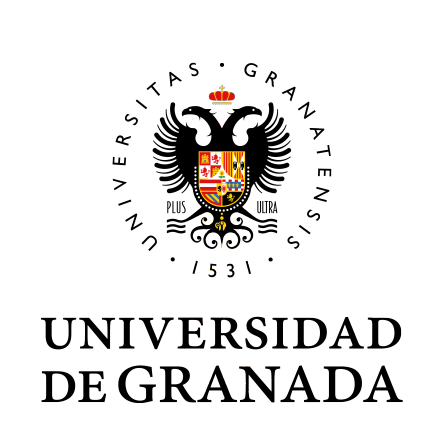
\includegraphics[scale=0.5]{img/ugr.png}\\

\textsc{\Large Aprendizaje Automático\\[0.2cm]}
\textsc{GRADO EN INGENIERÍA INFORMÁTICA}\\[1cm]

\noindent\rule[-1ex]{\textwidth}{1pt}\\[1.5ex]
\textsc{{\Huge TRABAJO 1\\[0.5ex]}}
\textsc{{\Large Cuestiones de Teoría\\}}
\noindent\rule[-1ex]{\textwidth}{2pt}\\[3.5ex]

\end{minipage}

\vspace{0.5cm}

\begin{minipage}{\textwidth}

\centering

\textbf{Autor}\\ {Vladislav Nikolov Vasilev}\\[2.5ex]
\textbf{Rama}\\ {Computación y Sistemas Inteligentes}\\[2.5ex]
\vspace{0.3cm}


\includegraphics[scale=0.3]{img/etsiit.jpeg}

\vspace{0.7cm}
\textsc{Escuela Técnica Superior de Ingenierías Informática y de Telecomunicación}\\
\vspace{1cm}
\textsc{Curso 2018-2019}
\end{minipage}
\end{titlepage}

\pagenumbering{arabic}
\tableofcontents
\thispagestyle{empty}				% No usar estilo en la pagina de indice

\newpage

\setlength{\parskip}{1em}

\section*{Ejercicio 1}
\addcontentsline{toc}{section}{Ejercicio 1}

\noindent Identificar, para cada una de las siguientes tareas, cuál es el problema, qué tipo de aprendizaje es el adecuado
(supervisado, no supervisado, por refuerzo) y los elementos de aprendizaje $(\mathcal{X} , f, \mathcal{Y})$ que deberíamos
usar en cada caso. Si una tarea se ajusta a más de un tipo, explicar como y describir los elementos para cada tipo.

\begin{enumerate}[label=\textit{\alph*})]
	\item Clasificación automática de cartas por distrito postal.
\end{enumerate}

\answer

El problema ante el que nos encontramos en este caso consiste clasificar cartas según su distrito postal. Posiblemente
sea un problema de clasificación donde hayan $k$ clases, una por cada código postal, así que el aprendizaje supervisado puede
ser la opción más efectiva para determinar a qué clase pertenece una carta.

El conjunto de datos de entrada $\mathcal{X}$ puede ser por ejemplo los datos del destinatario (su dirección, por ejemplo). El
conjunto de etiquetas $\mathcal{Y}$ que podríamos usar son $k$ etiquetas de números enteros, como por ejemplo $\lbrace 0, 1,
\dots , k \rbrace$, cada una de las cuáles se asocia con un distrito postal. La función $f$ sería alguna función tal que $f:
\; \mathcal{X} \mapsto \mathcal{Y}$.

\begin{enumerate}[resume,label=\textit{\alph*})]
	\item Decidir si un determinado índice del mercado de valores subirá o bajará dentro de un período de tiempo fijado.
\end{enumerate}

\answer

El problema en este caso consiste en predecir o decidir a partir de unos datos de entrada una clase (la de si subirá o bajará
el índice de mercado). Por tanto este problema se puede ver como una clasificación binaria $(0, 1)$ o $(-1, 1)$.

En el caso de los datos de entrada $\mathcal{X}$ podríamos utilizar valores del mercado y el tiempo. En el caso de los datos
de salida o etiquetas $\mathcal{Y}$ podríamos tener las etiquetas $(-1, 1)$, siendo $-1$ el caso de bajar el índice y $1$ el
de subir. Y por último, $f$ sería una función que relacione a $\mathcal{X}$ y a $\mathcal{Y}$ tal que $f: \; \mathcal{X}
\mapsto \mathcal{Y}$.

\begin{enumerate}[resume,label=\textit{\alph*})]
	\item Hacer que un dron sea capaz de rodear un obstáculo.
\end{enumerate}

\answer

El problema en este caso es hacer que un dron aprenda a esquivar un obstáculo rodeándolo. Como el objetivo no es clasificar
ninguna información, ni predecir ningún valor real ni buscar características o patrones en los datos, parece que el tipo
de aprendizaje más adecuado es el aprendizaje por refuerzo. Esto se podría hacer mediante un simulador en un ordenador, donde
se representaría el espacio donde se quiere entrenar al dron. Una vez entrenado en este simulador, se podría transferir todo
lo aprendido al dron y ver cómo se desempeña.

Como tal, el aprendizaje por refuerzo no tendría ni entradas $\mathcal{X}$, ni etiquetas de salida $\mathcal{Y}$ ni una
función $f$ para el aprendizaje, pero sí que tendría otra información que se correspondería con un Proceso de Decisión de
Markov (MDP), como por ejemplo un conjunto de estados, acciones, probabilidades de transicionar de un estado a otro, una
recompensa por transicionar de estado, etc.

\begin{enumerate}[resume,label=\textit{\alph*})]
	\item Dada una colección de fotos de perros, posiblemente de distintas razas, establecer
	cuántas razas distintas hay representadas en la colección.
\end{enumerate}

\answer

En este caso el problema consiste en encontrar patrones o características que permitan agrupar los datos (agrupar los perros
según su raza, para saber cuántas hay). Por tanto, al no saber a priori cómo se clasifican los datos, el aprendizaje no
supervisado sería la mejor opción para descubrir como se agrupan éstos.

En este caso, $\mathcal{X}$ son los datos de los que dispondríamos (las fotos de los perros), $\mathcal{Y}$ sería desconocido
ya que no sabemos qué clases hay (no sabemos las razas de perros) y $f$ sería una función de distribución condicional que se
quiere aprender con tal de intentar agrupar los datos.

\section*{Ejercicio 2}
\addcontentsline{toc}{section}{Ejercicio 2}

\noindent ¿Cuáles de los siguientes problemas son más adecuados para una aproximación por aprendizaje y cuáles más adecuados
para una aproximación por diseño? Justificar la decisión.

\begin{enumerate}[label=\textit{\alph*})]
	\item Determinar si un vertebrado es mamífero, reptil, ave, anfibio o pez.
\end{enumerate}

\answer

Este problema parece ser más adecuado para el diseño, ya que si se conocen qué características diferencian a los distintos
animales, no hace falta aprender nada, solo aplicarlas. Además, por lo general, el problema suele ser bien conocido, con lo
cuál la mayoría de características son conocidas, y solo haría falta ajustar unos pocos parámetros para distinguir ciertos
casos.

\begin{enumerate}[resume,label=\textit{\alph*})]
	\item Determinar si se debe aplicar una campaña de vacunación contra una enfermedad.
\end{enumerate}

\answer

Este problema parece que puede ser aproximado mejor por diseño que por aprendizaje, ya que es un problema conocido, que 
es la aplicación de una campaña de vacunas, y solo queremos ajustar algún parámetro, como por ejemplo sería el umbral de
personas enfermas desde el que se aplicaría. No haría falta aprender todo el modelo, solo ajustar ese dato.
cumplirse una condición que se aplique.

\begin{enumerate}[resume,label=\textit{\alph*})]
	\item Determinar perfiles de consumidor en una cadena de supermercados.
\end{enumerate}

\answer

Para este porblema lo mejor es el aprendizaje, el aprendizaje no supervisado en concreto. No conocemos a priori cuántos
perfiles hay y como distinguirlos, pero podemos aplicar alguna técnica de aprendizaje no supervisado con el objetivo de
encontrar patrones que permitan distinguir unos perfiles de otros y ver a cuál pertenece un individuo. 

\begin{enumerate}[resume,label=\textit{\alph*})]
	\item Determinar el estado anímico de una persona a partir de una foto de su cara.
\end{enumerate}

\answer

La mejor aproximación que se puede seguir en este caso es el aprendizaje, ya que como tal no conocemos exactamente
qué detalles de una expresión facial determinan el estado anímico. Si las supiésemos, podríamos simplemente codificar el
diseño de éstas, pero como no las sabemos, optaremos por aprender de los datos. Se puede seguir alguna técnica de aprendizaje
supervisado o no supervisado para determinar dichos detalles.

\begin{enumerate}[resume,label=\textit{\alph*})]
	\item Determinar el ciclo óptimo para las luces de los semáforos en un cruce con mucho tráfico.
\end{enumerate}

\answer

En este caso, la mejor aproximación que podemos seguir es el aprendizaje, y más concretamente, el aprendizaje por refuerzo.
Esto se debe a que se puede construir un simulador donde entrenar un semáforo mediante aprendizaje por refuerzo para que
aprenda cuál sería el ciclo óptimo de luces para un determinado cruce con mucho tráfico. Después, se podría trasladar
todo lo aprendido al semáforo.


\section*{Ejercicio 3}
\addcontentsline{toc}{section}{Ejercicio 3}

\noindent Construir un problema de \textit{aprendizaje desde datos} para un problema de clasificación de fruta en una
explotación agraria que produce mangos, papayas y guayabas. Identificar los siguientes elementos formales $\mathcal{X},
\mathcal{Y}, \mathcal{D}, f$ del problema. Dar una descripción de los mismos que pueda ser usada por un computador.
¿Considera que en este problema estamos ante un caso de etiquetas con ruido o sin ruido? Justificar las respuestas.

\answer

Vamos a suponer que nos encontramos ante un problema de clasificación, y por tanto, de aprendizaje supervisado. Para construir
nuestro modelo podemos considerar los siguientes elementos:

\begin{itemize}
	\item $\mathcal{X}$ sería el vector de características de las frutas. Podríamos considerar características tales como
	el \textbf{color}, la \textbf{forma}, el \textbf{tamaño} y la \textbf{textura}. 
	\begin{itemize}
		\item El \textbf{color} se podría codificar como una categoría, de tal forma que solo pudiese tomar un valor, como 
		por ejemplo 0 para el verde, 1 para el amarillo y 2 para el verde.
		\item La \textbf{forma}, al igual que el color, podría tomar un valor categórico, siendo 0 redonda y 1 ovalada.
		\item El \textbf{tamaño} puede ser también una variable categórica, tomando los valores 0 para pequeño y 1 para
		grande.
		\item La \textbf{textura} también puede verse como una variable categórica, pudiendo tomar los valores 0 para
		lisa y 1 para granulada.		
	\end{itemize}
	\item $\mathcal{Y}$ serían los valores de las etiquetas. Podríamos tener 0 para el \textbf{mango}, 1 para la
	\textbf{papaya} y 2 para la \textbf{guayaba}.
	\item $\mathcal{D}$ podría ser en este caso un conjunto de vectores de características con sus correspondientes etiquetas,
	es decir una muestra, con la cuál pordríamos entrenar nuestro modelo. Es muy importante que sea una muestra independiente
	(un elemento no condiciona a los otros) e idénticamente distribuida (cada elemento de la muestra tenga la misma
	probabilidad).
	\item $f$ sería nuestra función objetivo, una función desconocida que permitiese asignar las etiquetas a nuestras
	entradas, es decir, que $f: \; \mathcal{X} \mapsto \mathcal{Y}$.
\end{itemize}

En este caso podríamos encontrarnos ante un caso de etiquetas con ruido. Por ejemplo, puede que debido a factores que no
hayamos considerado a la hora de establecer las características usadas en $\mathcal{X}$ nos encontremos con que hayan dos
frutas con las mismas características, pero que sin embargo luego se hayan clasificado en distintas clases (como puede ser
que en algún caso haya habido algúna anomalía durante el crecimiento de una de las frutas y haga que tenga características
similares a las de una fruta de la otra clase).

\section*{Ejercicio 4}
\addcontentsline{toc}{section}{Ejercicio 4}

\noindent Suponga una matriz cuadrada A que admita la descomposición A = X\textsuperscript{T}X para alguna matriz X de
números reales. Establezca una relación entre los valores singulares de las matriz A y los valores singulares de X.

\answer

Vamos a partir de que la matriz $X$ puede descomponerse en valores singulares de la forma:

\begin{equation}
\label{eq:SVD}
	X = UDV^T
\end{equation}

\noindent donde encontramos que:

\begin{itemize}[label=\textbullet]
	\item $U$ es una matriz ortogonal, y por tanto, $U^{-1} = U^T$.
	\item $D$ es una matriz diagonal que contiene los valores singulares de $X$ en su diagonal principal ordenados de mayor
	a menor.
	\item $V$ es una matriz ortogonal, de forma que $V^{-1} = V^T$
\end{itemize}

Al sustituir los valores de $X$ en la descomposición original por la descomposición mostrada en (\ref{eq:SVD}), obtenemos que:

\begin{equation}
\label{eq:A_SVD}
	A = X^TX = (UDV^T)^T(UDV^T) = VDU^TUDV^T = VDDV^T = VD^2V^T
\end{equation}

Por tanto, al haber supuesto que la matriz $A$ se podía descomponer en $X^TX$, podemos suponer que el resultado obtenido en
(\ref{eq:A_SVD}) se corresponde con la descomposición en valores singulares de $A$. Como hemos partido sustituyendo $X$ por su
descomposición en valores singulares, y sabiendo que los valores propios de la matriz $X$ están contenidos en $D$, entonces
podemos decir que los valores propios de $A$ son los de $X$ al cuadrado.

\section*{Ejercicio 5}
\addcontentsline{toc}{section}{Ejercicio 5}

\noindent Sean \textbf{x} e \textbf{y} dos vectores de características de dimensión $M \times 1$. La expresión

\[ \cov(\mathbf{x}, \mathbf{y}) = \frac{1}{M} \sum_{i = 1}^M(x_i - \overline{x})(y_i - \overline{y})\]

\noindent define la covarianza entre dichos vectores, donde $\overline{z}$ representa el valor medio de los
elementos de \textbf{z}. Considere ahora una matriz X cuyas columnas representan vectores de características.
La matriz de covarianzas asociada a la matriz $\text{X} = (\text{\textbf{x}}_1, \text{\textbf{x}}_2, \dots ,
\text{\textbf{x}}_N)$ es el conjunto de covarianzas definidas por cada dos de sus vectores columnas. Es decir,

\begin{equation}
\label{eq:cov}
\cov(\mathbf{X})
=
\left(
{
\begin{array}{cccc}
	\cov(\mathbf{x}_1,\mathbf{x}_1) & \cov(\mathbf{x}_1,\mathbf{x}_2) & \cdots & \cov(\mathbf{x}_1,\mathbf{x}_N) \\
	\cov(\mathbf{x}_2,\mathbf{x}_1) & \cov(\mathbf{x}_2,\mathbf{x}_2) & \cdots & \cov(\mathbf{x}_2,\mathbf{x}_N) \\
	\cdots & \cdots & \cdots & \cdots \\	
	\cov(\mathbf{x}_N,\mathbf{x}_1) & \cov(\mathbf{x}_N,\mathbf{x}_2) & \cdots & \cov(\mathbf{x}_N,\mathbf{x}_N)
\end{array}
}
\right)
\end{equation}


Sea $\mathbf{1}^T = (1, 1, \dots , 1)$ un vector $M \times 1$ de unos. Mostrar que representan las siguientes expresiones:

\begin{enumerate}[label=\textit{\alph*})]
	\item $E1 = \mathbf{1}\mathbf{1}^T$X
\end{enumerate}

\answer

Sabiendo que $\mathbf{1}$ es un vector $M \times 1$, $\mathbf{1}^T$ es un vector $1 \times M$ y que X es una matriz $M \times
N$, podemos aplicar la propiedad asociativa para multiplicar $\mathbf{1}\mathbf{1}^T$, con lo cuál obtendríamos una matriz
$M \times M$ de unos. Por tanto, al multiplicar ahora la matriz de unos por X, como éstas tienen dimensiones $M \times M$ y
$M \times N$ respectivamente, obtenemos una matriz $M \times N$ en la que todos los elementos de una columna son la suma de
los elementos de esa columna. Es decir, para la columna $j$-ésima de la matriz resultado (de forma que $j \in [1, 2, \dots ,
N]$), el elemento $i$-ésimo de esa columna (de manera que $i \in [1, 2, \dots, M]$), sería la suma de todos los elementos de
la columna $j$-ésima de la matriz X original.  

\begin{enumerate}[resume,label=\textit{\alph*})]
	\item $E2 = (\text{X} - \frac{1}{M}E1)^T(\text{X} - \frac{1}{M}E1)$
\end{enumerate}

\answer

Si comenzamos a operar dentro de los paréntesis, podemos ver que la primera operación que podemos realizar es el producto
de $E1$ por un escalar.

Como sabemos de antes, $E1$ es una matriz en la que todos los elementos de una columna son la suma de todos los elementos de
la columna correspondiente en X. Al realizar el producto por un escalar, en este caso $\frac{1}{M}$, realmente estamos
calculando, para cada elemento de la matriz, la media, ya que como se ha dicho antes, cada elemento de una columna es el
sumatorio de los $M$ elementos de la misma columna de X. Con lo cuál, ahora cada elemento de una columna contendrá la media
de la suma de los elementos de la misma columna de X. Llamémos a esta matriz $\overline{X}$.

La siguiente operación que podemos realizar, aun dentro de los paréntesis, es X$- \overline{X}$ (lo que se corresponde con
X$- \frac{1}{M}E1$). Con esto, lo que obtenemos es la diferencia de cada elemento de X con respecto a la media, es decir
su desviación con respecto a la media. Esto se puede ver de la siguiente forma:

\begin{equation}
\begin{split}
X - \overline{X} &=
\left(
{
\begin{array}{cccc}
	x_{11} & x_{12} & \cdots & x_{1N} \\
	x_{21} & x_{22} & \cdots & x_{2N} \\
	\cdots & \cdots & \cdots & \cdots \\
	x_{M1} & x_{M2} & \cdots & x_{MN}
\end{array}
}
\right)
-
\left(
{
\begin{array}{cccc}
	\overline{x}_{1} & \overline{x}_{2} & \cdots & \overline{x}_{N} \\
	\overline{x}_{1} & \overline{x}_{2} & \cdots & \overline{x}_{N} \\
	\cdots & \cdots & \cdots & \cdots \\
	\overline{x}_{1} & \overline{x}_{2} & \cdots & \overline{x}_{N}
\end{array}
}
\right) \\
&=
\left(
{
\begin{array}{cccc}
	x_{11} - \overline{x}_{1} & x_{12} - \overline{x}_{2} & \cdots & x_{1N} - \overline{x}_{N} \\
	x_{21} - \overline{x}_{1} & x_{22} - \overline{x}_{2} & \cdots & x_{2N} - \overline{x}_{N} \\
	\cdots & \cdots & \cdots & \cdots \\
	x_{M1} - \overline{x}_{1} & x_{M2} - \overline{x}_{2} & \cdots & x_{MN} - \overline{x}_{N}
\end{array}
}
\right)
\end{split}
\end{equation}

Habiendo calculado esto, ahora solo nos queda calcular el producto. La traspuesta de la matriz que se ha obtenido
anteriormente es la siguiente (llamemos X$_{dev}$ a esta matriz, para darle un nombre):

\begin{equation}
\label{eq:x1t}
X_{dev}^T = 
\left(
{
\begin{array}{cccc}
	x_{11} - \overline{x}_{1} & x_{21} - \overline{x}_{1} & \cdots & x_{M1} - \overline{x}_{1} \\
	x_{12} - \overline{x}_{2} & x_{22} - \overline{x}_{2} & \cdots & x_{M2} - \overline{x}_{2} \\
	\cdots & \cdots & \cdots & \cdots \\
	x_{1N} - \overline{x}_{N} & x_{2N} - \overline{x}_{N} & \cdots & x_{MN} - \overline{x}_{N}
\end{array}
}
\right)
\end{equation}

Al realizar la multiplicación ($X_{dev}^TX_{dev}$), lo que obtenemos en realidad no es nada más ni nada menos que una
expresión parecida a la covarianza que se puede ver en (\ref{eq:cov}). Es decir, al multiplicar cada fila de  X$_{dev}$ por
cada columna de X, lo que se obtiene es una sumatoria de $(x_{ij} - x_j)(x_{ji} - x_j)$, para $i \in [1, 2, \dots, M]$ y $j
\in [1, 2, \dots, N]$ (sabiendo que la matriz X es $M \times N$). Lo único que pasa es que cada elemento está multiplicado por
$M$, ya que no se ha realizado en ningún momento la división. Por tanto, como $M$ multiplica a cada elemento, se puede sacar
fuera de esta expresión y dejarlo como un producto de matriz por escalar, pudiendo ahora sí expresar el resultado en función
de la covarianza. Por tanto, obtenemos que el valor de $E2$ es el siguiente:

\begin{equation}
	E2 = M \cov(\text{X})
\end{equation}

\section*{Ejercicio 6}
\addcontentsline{toc}{section}{Ejercicio 6}

\noindent Considerar la matriz \textbf{hat} definida en regresión, Ĥ = X(X$^\text{T}$X)$^{-1}$X$^\text{T}$, donde X es la
matriz de observaciones de dimensión $N \times (d + 1)$, y X$^\text{T}$X es invertible. Justificar las respuestas.

\begin{enumerate}[label=\textit{\alph*})]
	\item ¿Que representa la matriz Ĥ en un modelo de regresión?
\end{enumerate}

\answer

\begin{enumerate}[resume,label=\textit{\alph*})]
	\item Identifique la propiedad más relevante de dicha matriz en relación con regresión lineal.
\end{enumerate}

\answer

La propiedad más importante de esta matriz es la idempotencia. Es decir, se da que Ĥ$^2 = $ Ĥ.

\section*{Ejercicio 7}
\addcontentsline{toc}{section}{Ejercicio 7}

\noindent La regla de adaptación de los pesos del Perceptron (\textbf{w}$_{new}$ = \textbf{w}$_{old}$ + $y$\textbf{x}) tiene
la interesante propiedad de que mueve el vector de pesos en la dirección adecuada para clasificar \textbf{x} de forma
correcta. Suponga el vector de pesos \textbf{w} de un modelo y un dato \textbf{x}$(t)$ mal clasificado respecto de dicho
modelo. Probar matematicamente que el movimiento de la regla de adaptación de pesos siempre produce un movimiento de
\textbf{w} en la dirección correcta para clasificar bien \textbf{x}$(t)$.


\section*{Ejercicio 8}
\addcontentsline{toc}{section}{Ejercicio 8}

\section*{Ejercicio 9}
\addcontentsline{toc}{section}{Ejercicio 9}

\section*{Ejercicio 10}
\addcontentsline{toc}{section}{Ejercicio 10}

\newpage

\begin{thebibliography}{5}

\bibitem{nombre-referencia}
Texto referencia
\\\url{https://url.referencia.com}

\end{thebibliography}

\end{document}

